\chapter{Systemanalyse}\label{sec:simulation}
Nachdem nun im vorherigen Kapitel ein erstes Modell mitsamt Aktuatorik entwurfen wurde, soll nun überprüft werden, ob dieses unter Last zum einen genügend Festigkeit besitzt und zum anderen, ob die Aktuatorik auch die entsprechenden Leistungen liefern kann. Auf Basis dieser Analysen werden anschließend Optimierungen der in Kapitel \ref{sec:modellentwurf} getroffenen Entscheidungen vorgenommen.


\section{FEM-Analyse}
Solid Edge bietet direkt das integrierte FEM-Program "NX Nastran" an, was einen schnellen Designzyklus von berechnen und Modell bearbeiten ermöglicht. Für eine effiziente FEM-Analyse werden die Modellvarianten zunächst vereinfacht, indem die Verrundungen und Anschrägungen der Wände entfernt werden. Auch einige der steilen Spitzen der Pfeilung werden abgerundet, da diese bei der Vernetzung nur zu Problemen führt und die Belastungen im Material so gut wie gar nicht verändern.

Bevor dir Kräfte aus Formel \ref{eq_Fmax} und \ref{eq_Fmax2} auf die Geometrie angewandt werden können, müssen sie noch aus dem körperfesten in ein Grid Fin festes Koordinatensystem übertragen werden. Dieses ist in Abbildung \ref{abb_gitter} dargestellt und wurde so definiert, dass die Kräfte $F_2$ und $F_3$ genau normal auf den Gitterwänden stehen, sodass sie sich einfach in der FEM-Analyse implementieren lassen. $F_1$ ist parallel zur Sehne und kann somit, genau wie die anderen beiden Kräfte, gleichmäßig auf alle Flächen verteilt werden, die eine Normale haben, die zum Teil in diese Richtung zeigt.
\begin{figure}[h] 
	\centering
	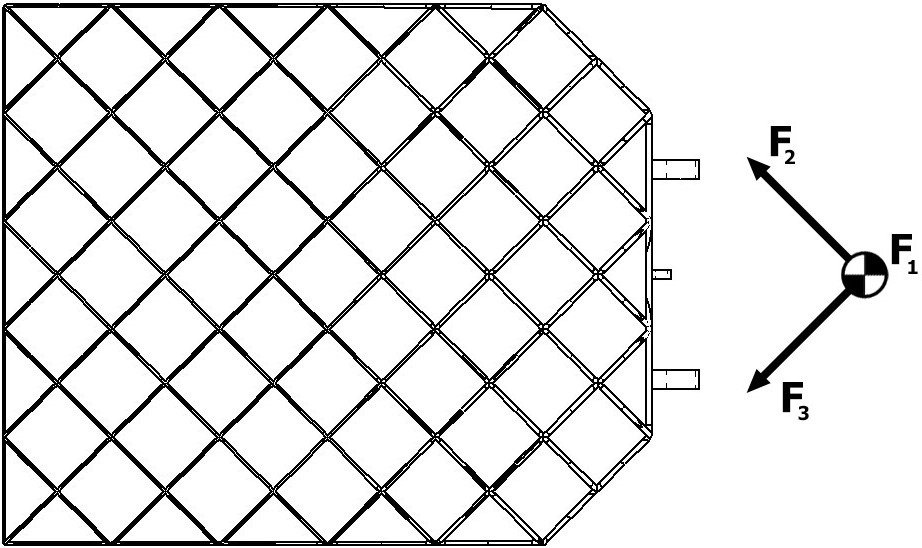
\includegraphics[width=0.9\textwidth]{Gitter.jpg}
	\caption{Kräfte im Grid Fin festen Koordinatensystem}
	\label{abb_gitter}
\end{figure}\\
Somit ergeben sich die Kräfte für die einzelnen Grid Fins zu:
\begin{table}[h]
	\centering
	\begin{tabular}{c||c|c|c|c}
		&D1&R1&D2&R2\\
		\hline
		$F_1/$N&$413,5$&$389,3$&$389,3$&$413,5$\\
		$F_2/$N&$6276,0$&$4970,8$&$-4970,8$&$-6276,0$\\
		$F_3/$N&$4934,0$&$6474,2$&$-6474,2$&$-4934,0$\\
	\end{tabular}
\end{table}
\subsection{Optimierung der Halterung}
Bei beiden Pfeilungstypen lässt sich für alle Lastfälle sofort erkennen, dass es zu massiven Lastspitzen an der Halterung kommt. Währenddessen bleiben die Werte im Gitter deutlich niedriger. Der Grund für die hohen Spannungen an der Einspannung ist die ungünstige Lage in der Mitte der Wände anstatt der Schnittstellen, Somit bilden sich vergleichsweise hohe Biegemomente in den Wänden aus. Dieser ungünstige Kraftfluss wird durch die scharfen Kanten weiter verschlimmert. Um nun diese Spannungsspitzen zu vermeiden, sollte, neben einer Abrundung der Kanten, die Position der Halterungen verändert werden.

Da sich die Anbringung der Halterungen genau ein der Mitte Zelle befinden, auch wenn sie in diesem Fall halbiert sind, lassen sie sich entweder tangential oder normal zum Raketenkörper verschieben, um sie auf einen Schnittpunkt der Wände zu legen. Soll Halterung B nicht in zwei Teile aufgeteilt werden, so kommt nur eine Bewegung senkrecht zum Körper in Frage. Anstatt die Halterung nun in das Gitter hinein zu legen, was zu einer Verkleinerung der durschdtrömten Querschnittfläche führen würde und somit geringer Normalkräfte, werden zwei der Wände weiter fortgesetzt. Diese schneiden sich dann in der Mitte, wo die Halterung B platziert wird. Die Halterung wird jedoch nicht direkt an der Schnittstelle konstruiert, sondern noch ein bisschen weiter vom Gitter entfernt, sodass die Kraft gradliniger über die Beiden Hubstangen geleitet werden kann.

Für die Halterungen A passiert das gleiche. Die nebenliegenden Gitterwänder werden bis zu ihrer Schnittstelle fortgesetzt. Im Gegensatz zur Halterung B befindet sich jedoch direkt hier die Bohrung, an der das Grid Fin montiert werden soll.
\section{Betriebssimulation}
Für Überprüfung der Aktuatorik wird eine Betriebssimulation in Simulink durchgeführt.
Im Zentrum steht die Differenzialgleichung der Verdrehung des Grid Fins $\delta$, die abhängig vom Moment, dass der Motor liefert, ist. Dieses Moment lässt sich aus der Gleichung
\begin{equation}
	n =k_nU-\frac{\Delta n}{\Delta M}M_{Motor}
\end{equation}
berechnen. $n$ ist hierbei die Drehzahl des Motors, $U$ die Spannung, die am Motor angelegt wird, $\frac{\Delta n}{\Delta M}$ die Steigung der Motorkennlinie und schlussendlich $M_{Motor}$ als das vom Motor erzeugte Moment. Die Größen $k_n$ und $\frac{\Delta n}{\Delta M}$ sind konstante Kenngrößen des Motors und werden vom Herstellen angegeben. Die Drehzahl hingeben ergibt sich aus der Differenzialgleichung des Systems. Das Moment wird anschließend nur noch durchs Getriebe zum Antriebsmoment $M_{Antrieb}$ übersetzt und dann an die Differenzialgleichung übergeben.
\\~\\
Diese ergibt sich nun aus dem Momentengleichgewicht zu:
\begin{equation}
	I\ddot{\delta} = M_{Antrieb} - M_{m, \delta}\delta - M_{R, \dot{\delta}}\dot{\delta}
\end{equation}
Das Trägheitsmoment setzt sich aus dem des Motors, des Getriebes und des Grid Fins zusammen. Dabei muss das Trägheitsmoment des Motors noch mit der Übersetzung des Getriebes multipliziert werden, da dieser um jenen Faktor stärker beschleunigt. Das aerodynamische Moment wird als linear vom Steuerwinkel abhängig angenommen. Somit ergibt sich $M_{m, \delta} = M_{m, max}/\delta = 4,455Nm/^\circ$. Das Reibmoment setzt sich aus der Reibung des Motors, des Getriebes und der Lagerung zusammen.

Während die Motorspannung $U$ als Eingangsgröße für das System geregelt wird, ergibt sich der Sollwert für den Steuerwinkel aus der Bedingung den auftretenden Schwingungen ausgleichen zu können. Da also eine solche komplette Schwingung innerhalb von $T = 0,73$s stattfinden soll, wird der Sollwert für den Steuerwinkel bis $t = 1/4T$ auf $\delta = 20^\circ$ gesetzt. Danach springt der Wert auf $\delta = -20^\circ$ und ab $t = 3/4T$ soll Steuerwinkel wieder auf $\delta = 0^\circ$ zurück gehen, wo er auch gestartet ist.
\section{Systemoptimierung}

\section{Systembewertung}

\section{Fazit}